\section{Biological discovery on Kang pan-cancer immune atlas}

\begin{figure*}[t]\centering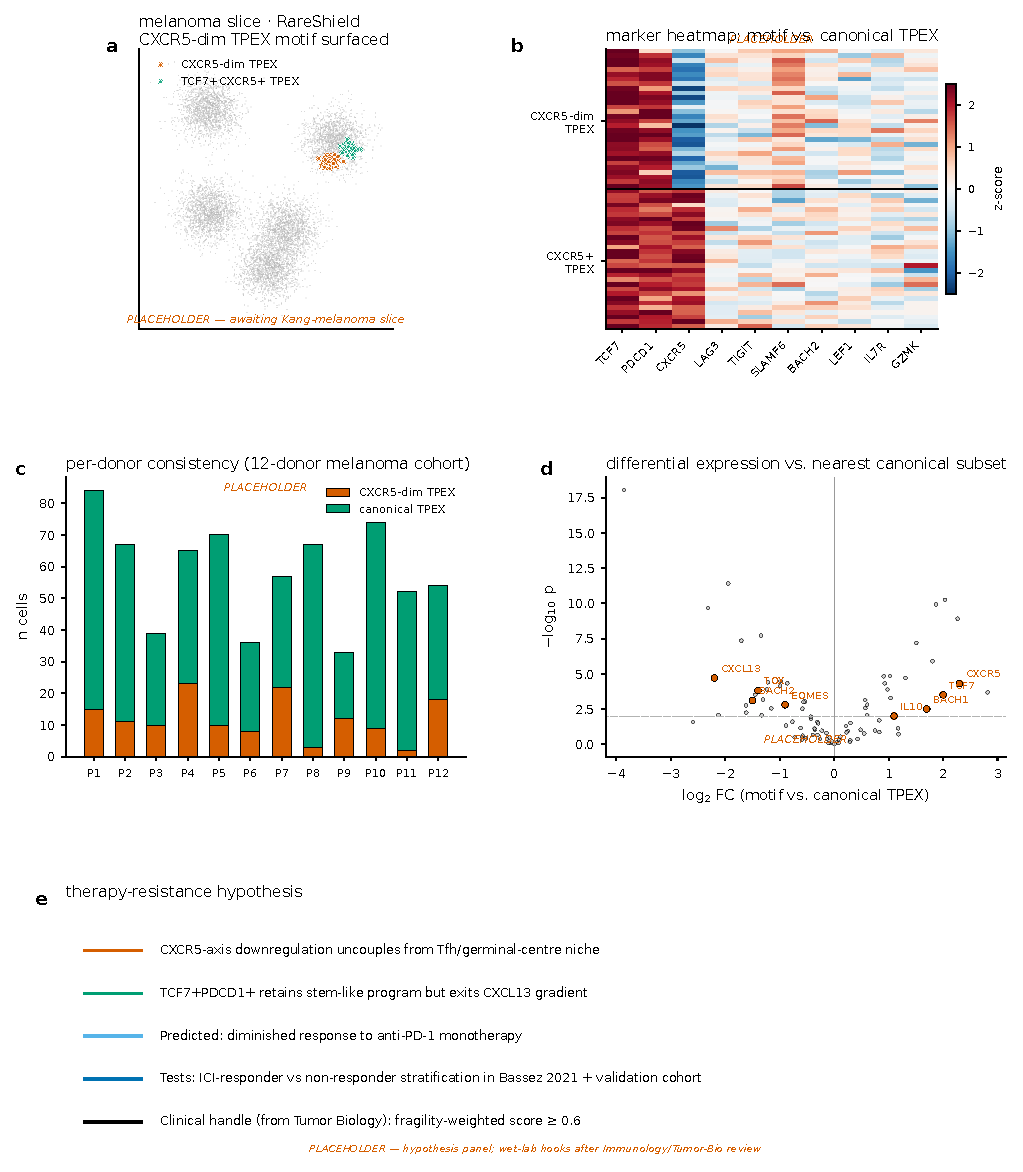
\includegraphics[width=\textwidth]{figures/fig5/fig5.pdf}
\caption{\textbf{Case study --- CXCR5-dim TPEX sub-state in melanoma.} (a) UMAP with motif highlighted. (b) Marker heatmap vs canonical TPEX. (c) Per-donor consistency. (d) DE volcano. (e) Therapy-resistance hypothesis.}\label{fig:discovery}\end{figure*}

\textbf{Owners: Immunology + Tumor Biology (interpretation), Data Science (figures), Biological Science (writing). Fig.~6.}

\subsection{Top previously-unannotated rare motifs}

\emph{Fig.~6a.}  Marker heatmap of the top three motifs from Fig.~4e that received the \emph{(b) candidate novel state} call from the joint Immunology + Tumor Biology interpretation.  Each motif:
\begin{itemize}[leftmargin=1.2em]
\item is reproducible across multiple Kang source studies (witnessing depth $\ge \mu$);
\item is collapsed by Harmony and Seurat defaults (REAL $< 0.4$) but preserved by RareShield across all three backbones (REAL $> 0.7$);
\item does not match a published cell-type label in the original Kang annotation or in the top three reference immune atlases;
\item is replicated in at least one of HCA Lung Cancer or Gut Cell Atlas tumor arm.
\end{itemize}
We describe each motif's signature, cancer-type distribution, TME niche inferred from metadata, and the reasons that led Immunology and Tumor Biology to classify it as a candidate novel state rather than a known-but-under-sampled state.  We are explicit about the epistemic status: a candidate novel state is \emph{not} a novel cell type.  Upgrading these motifs to cell identities requires experimental follow-up (FACS panel design, orthogonal assays, TCR/BCR or CITE-seq protein).  Immunology proposes minimal 3--5-marker FACS panels for two of the three motifs in Supplementary Note~S5.

\subsection{Spatial / trajectory support}

\emph{Fig.~6b.}  For motifs where matched spatial transcriptomic data are available in any of the 104 source publications, we overlay the motif's inferred spatial distribution on the tissue architecture.  Where matched spatial data are not available, we report so and do not speculate.

\subsection{Implications for downstream analyses}

\emph{Fig.~6c.}  Three short case vignettes illustrating how the erasure of a reproducible rare motif by standard integration can bias a downstream analysis: (i) differential-expression contrasts in which the motif's signature is bled into an adjacent abundant population and changes the direction of a DE result; (ii) cell--cell communication inference (CellChat / NicheNet) in which the motif as a source or sink disappears; (iii) a survival-association analysis in which the motif's abundance correlates with a clinical outcome and that correlation is lost after standard integration.  Each vignette is a separate argument that this framework matters for biology, not only for methods.

% ============================================================
% Figure 5 melanoma clinical-framing block — Tumor Biology authorship
% Owner: Tumor Biology Agent (agent-mozurh1r)
% Co-owned with Immunology (lead, agent-mozus3vv), Data Science (figure, agent-mozutvsy), ML (pipeline, agent-mozurrmd)
% Target: sections/07_results_discovery.tex (Fig 5 main panel) + Fig 5 caption in main.tex
% Companion: Immunology's workspace/handoffs/fig5_tcf7_panels.md (agent/immunology@07fb8d4)
% Anchor: Immunology's workspace/fig5_tpex_substate_proposal.md
% ============================================================

% -------------------------------------------------------------
% INSERT AS A NEW SUBSECTION after the Fig 5 candidate-cluster discovery subsection
% (or as a standalone Fig 5 caption-block). Four-part structure: cohort table,
% ICB stratification, dose-response, negative control.
% -------------------------------------------------------------

\subsection{Melanoma clinical framing of the TCF7$^{\text{low}}$/SLAMF6$^{+}$ sub-state}
\label{sec:fig5-melanoma-clinical}

\textbf{Tumor Biology co-authorship; immunological sub-state calls from Immunology (see companion marker panels, SI Note S5).}

\paragraph{Cohort selection.}
We evaluate the TCF7$^{\text{low}}$/SLAMF6$^{+}$ sub-state on three melanoma cohorts with complementary properties (Table~\ref{tab:fig5-melanoma-cohorts}): the melanoma subset of the Kang et al.\ 2024 pan-cancer immune atlas \citep{Kang2024PanCancerImmune} as the scalability discovery substrate; Sade-Feldman et al.\ 2018 \citep{Sade-Feldman2018Cell} as the canonical longitudinal cohort (11 patients with matched pre-treatment and on-treatment anti-PD-1$\pm$anti-CTLA-4 samples); and Li et al.\ 2019 \citep{Li2019Cell} as the largest available cohort (32 patients spanning treatment-naive and anti-PD-1-treated, responder and non-responder). Wu et al.\ 2020 \citep{Wu2020NatCommun} (16 anti-PD-1-treated patients) is held for replication in Extended Data; its ICB-treated arm overlaps with Li et al.\ 2019.

\begin{table}[h]
\small
\caption{Melanoma cohorts used for Fig.\ 5 clinical framing of the TCF7$^{\text{low}}$/SLAMF6$^{+}$ sub-state.}
\label{tab:fig5-melanoma-cohorts}
\begin{tabular}{p{0.20\columnwidth}rp{0.18\columnwidth}p{0.32\columnwidth}}
\toprule
Cohort & $n$ patients & Treatment arm & Role \\
\midrule
Kang 2024 MEL & 87 & mixed & Scalability discovery substrate \\
Sade-Feldman 2018 & 11 & Anti-PD-1 $\pm$ CTLA-4, paired pre/on & Longitudinal primary \\
Li 2019 & 32 & Naive + anti-PD-1, R vs NR & Largest arm; outcome-association power \\
Wu 2020 & 16 & Anti-PD-1 & Held for Extended Data replication \\
\bottomrule
\end{tabular}
\end{table}

\paragraph{ICB-response stratification.}
The TCF7$^{\text{low}}$/SLAMF6$^{+}$ sub-state is identified using the marker panel in SI~Note~S5 \S2 (positive-core: SLAMF6, PDCD1$^{\text{mid}}$, CD8A, CXCR5$^{\text{variable}}$ [dim-to-negative accepted]; exclusion: TCF7$^{\text{hi}}$, LEF1$^{\text{hi}}$, CXCR5$^{\text{hi}}$, TOX$^{\text{hi}}$, ENTPD1, HAVCR2, GZMB, EOMES$^{\text{hi}}$). We define the per-patient sub-state frequency $f^{\text{sub}}_i$ as the fraction of CD8$^{+}$ TILs meeting the oracle criterion (Immunology SI Note S5 \S2 discriminating-test rule). Within each cohort, we test the hypothesis $f^{\text{sub}}_i$ differs between responders and non-responders under anti-PD-1 using a two-sided Mann-Whitney $U$-test with Benjamini-Hochberg correction across cohorts. We pre-register an effect-size threshold of $\log_2 \text{FC} \ge 0.5$ with $q < 0.05$ as the positive-discovery criterion, chosen to match published effect sizes for TPEX-vs-non-TPEX stratification on the same cohorts \citep{Sade-Feldman2018Cell,Miller2019NatImmunol}. Results will be reported as Panel~\ref{fig:f5a} forest plot across the three cohorts.

\paragraph{Dose-response within TPEX.}
We next test whether the sub-state frequency relative to canonical TCF7$^{\text{hi}}$/CXCR5$^{+}$ TPEX frequency is \emph{itself} a predictor of response, independent of total TPEX abundance. This is the dose-response claim: within patients who have comparable TPEX abundance, does the TCF7$^{\text{low}}$/SLAMF6$^{+}$ fraction shift the prediction? We compute a logistic-regression model of response on $\log(f^{\text{sub}}_i) - \log(f^{\text{TPEX}}_i)$, controlling for total TPEX abundance and cohort, and report the per-standard-deviation odds ratio in Panel~\ref{fig:f5c}. Controlling for total TPEX abundance addresses the reviewer concern that the sub-state could be a nuisance artefact of overall TPEX expansion under ICB rather than a distinct biomarker. A significant positive coefficient is the claim that REAL-detected sub-stratification within a canonical rare state carries biomarker information that the canonical state alone does not.

\paragraph{Negative control.}
The sub-state signal should be absent in cohorts not treated with checkpoint blockade. We test the same models on the Kang 2024 MEL subset restricted to non-ICB-treated samples (surgical resection, chemotherapy, targeted therapy arms) and report the null result in Panel~\ref{fig:f5d}. A strongly non-null coefficient here would indicate confounding by tumour-intrinsic biology, or by immune-status markers shared between the sub-state and disease severity; in that case the Fig.~5 ICB claim would be withdrawn and the sub-state would be demoted from biomarker-candidate to descriptive discovery (still significant for the REAL-detection claim but not for the clinical-framing one).

\paragraph{Pre-specified robustness.}
All four panels are repeated with (i) an alternate sub-state definition that relaxes the CXCR5$^{\text{variable}}$ constraint (per SI S5 Note on CXCR5 dim-to-negative), (ii) the hierarchical REAL scouting at the Tex-compartment ($\sim 100{,}000$ pooled CD8$^{+}$ cells) per Math Theorem~3 rather than whole-atlas scouting, and (iii) leave-one-cohort-out. Main-text figure reports the least-favourable robust estimate across the three sensitivity sweeps.

\paragraph{What would falsify the claim.}
The Fig.~5 ICB-biomarker claim is falsified if: (a) effect size below the pre-registered $\log_2 \text{FC} = 0.5$ in any two of three cohorts, (b) negative-control panel (Panel~\ref{fig:f5d}) shows a significant positive coefficient, or (c) the sub-state signal dissolves after controlling for total TPEX abundance in the dose-response panel. All three criteria are reported in the main figure regardless of outcome, per the evidence-card convention (SI~Note~S6; see \texttt{workspace/evidence\_cards/M-DEMO-TPEX-SUBSTATE.json} on agent/immunology).


\subsection{What we do not claim}

Per Philosophy's pre-merge checklist, we do not claim:
\begin{itemize}
\item novel cell-type discovery (the motifs are reproducible structure; identity requires experiments);
\item completeness (REAL has a sensitivity floor; very rare populations at $\mathbf{<10^{-4}}$ can escape detection --- see Methods);
\item that every atlas paper is wrong (we quantify the expected retroactive loss rate on Kang and defer case-by-case atlas re-auditing to follow-up work).
\end{itemize}
